\documentclass{../cheat}
\title{Digital Image Processing}
\author{ma.mehralian}

\newenvironment{mask}
	{\renewcommand{\tabcolsep}{3pt} 
		\begin{tabular}{| >{\centering}p{10pt}| >{\centering}p{10pt} | p{10pt} | } }
	{\end{tabular}}

\begin{document}
\begin{multicols}{3}
	\section{Digital Image Fundamentals}
	\subsection{Light and the Electromagnetic Spectrum}
	$\lambda=\frac{c}{\nu}$
	$\lambda$ Wavelength, $\nu$ Frequency, $c$ the speed of light
	
	Electromagnetic Spectrum
	
	p45 chromatic, lumin ...
	
	image cordinate and axies\\
	
	contrast
	\subsection{Neighbors and Connectivities}
	\textbf{Neighbors of Pixel}
	\begin{itemize}[nolistsep, leftmargin=1em]
		\item \textbf{4-neighbors ($N_4(p)$):} $(x-1,y)$, $(x+1,y)$, $(x,y-1)$, and $(x,y+1)$
		\item \textbf{8-neighbors($N_8(p)$):} $N_4(p)$+ diagonal directions $(x-1,y-1)$, $(x-1,y+1)$, $(x+1,y-1)$ and $(x+1,y+1)$
	\end{itemize}
	\textbf{Connectivity}
	\begin{itemize}[nolistsep, leftmargin=1em]
		\item {\bf 4-connected} Two pixels $p$ and $q$ are 4-connected if they are 4-neighbors and
		$p \in V$ and $q \in V$;
		
		\item {\bf 8-connected}	Two pixels $p$ and $q$ are 8-connected if they are 8-neighbors and 
		$p \in V$ and $q \in V$;
		
		\item {\bf mixed-connected} Two pixels $p$ and $q$ are mix-connected if
		\begin{itemize}[nolistsep, leftmargin=1em]
			\item $p$ and $q$ are 4-connected, {\bf or}
			\item $p$ and $q$ are 8-connected {\bf and} not 4-connected through a third 
				pixel ($N_4(p) \cap N_4(q) \not\subset V$)
		\end{itemize}
	\end{itemize}
	
	\textbf{Distances}
	\begin{itemize}
		\item \textbf{Euclidean distance}:\\
		$D_E(p,q)=\sqrt{(x-u)^2+(y-v)^2}=[|x-u|^2+|y-v|^2]^{1/2}$
		\item \textbf{City-block distance}:\\
		$D_4(p,q)=|x-u|+|y-v|=[|x-u|^1+|y-v|^1]^{1/1}$
		\item \textbf{Chess-board distance}:\\
		$D_8(p,q)=max\{|x-u|,|y-v|\}=[|x-u|^\infty+|y-v|^\infty]^{1/\infty}$
		\item \textbf{General distance definition}:\\
		$D(p,q)=[|x-u|^L+|y-v|^L]^{1/L}$
	\end{itemize}
	
	 \hfill $D_4=$
	$\begin{matrix}
		4	&  3	&  2	&  3	&  4	\\
		3	&  2	&  1	&  2	&  3	\\
		2	&  1	&  0 	&  1	&  2	\\
		3	&  2	&  1	&  2	&  3	\\
		4	&  3	&  2	&  3	&  4	\\	
	\end{matrix}$
	\hfill $D_8=$
	$\begin{matrix}
		2	&  2	&  2	&  2	&  2	\\
		2	&  1	&  1	&  1	&  2	\\
		2	&  1	&  0 	&  1	&  2	\\
		2	&  1	&  1	&  1	&  2	\\
		2	&  2	&  2	&  2	&  2	
	\end{matrix}$\hfill \null

	
	\section{Transformations and Spatial Filtering}
	??? deference between correlation and convolution (180' rotation)
	
	Gamma correction : $y=A x^\gamma$
	
	\section{Filtering in Frequency Domain}
	++++ mesale tasviri az aliasing charkhe machine +++++
	
	Fourier Series of a function $f(t)$ with period $T$:\\
	$f(x)=\sum_{n=-\infty}^\infty c_n\ e^{2\pi i(n/T) x} $\\
	and \\
	$c_n = \frac{1}{T} \int_{-T/2}^{T/2} f(x)\ e^{-2\pi i(n/T) x} dx.$
	
	Fourier Transform (1D):\\
	$F(\omega) = \int_{-\infty}^\infty f(x)\ e^{- 2\pi i x \omega}\,dx$\\
	Inverse Fourier Transform (1D):\\
	$f(x) = \int_{-\infty}^\infty F(\omega)\ e^{2 \pi i \omega x}\,d\omega$\\
	
	
	Fourier Transform (2D):\\
	$F(\omega_x,\omega_y) = \int_{-\infty}^\infty f(x,y)\ e^{- 2\pi i (x \omega_x+y \omega_y)}\,dxdy$\\
	Inverse Fourier Transform (2D):\\
	$f(x,y)= \int_{-\infty}^\infty F(\omega_x,\omega_y)\ e^{- 2\pi i (x \omega_x+y \omega_y)}\,d\omega_x d\omega_y$
	
	
	\begin{tabularx}{\columnwidth}{| X	 | X |}
		\hline
		Function & Fourier transform\\
		\hline
		$f(x)$ & $F(\omega)$\\
		\hline
		$a.f(x)+b.g(x)$ & $a.F(\omega)+b.G(\omega)$\\
		\hline
		$f(x - a)$  & $e^{-2\pi i a \omega} F(\omega)$ \\
		\hline
		$e^{2\pi i a x} F(x)$ & $F(\omega-a)$\\
		\hline
		$f(ax)$ & $\frac{1}{a}F(\frac{\omega}{a})$\\
		\hline
		$f(x)*h(x)$ & $F(\omega)H(\omega)$\\
		\hline
		$f(x)h(x)$ & $F(\omega)*H(\omega)$\\
		\hline
		$\delta(x)$ & 1 \\
		\hline
		$e^{i a x}$ & $\delta(\omega-\frac{a}{2\pi})$ \\
		\hline
		$u(x)$ & $\frac{1}{2}(\frac{1}{i\pi \omega}+\delta (\omega))$ \\
		\hline
		$rect(x)$ & $sinc(\omega)$ \\
		\hline
		$sinc(x)$ & $rect(\omega)$ \\
		\hline
		$tri(x)$ & ${sinc}^2(\omega)$ \\
		\hline
		${sinc}^2(x)$ & $tri(\omega)$ \\
		\hline
	\end{tabularx}
	
	
	convolution theorem: \\
	
	4.6.2 -> transformation and rotation
	
	4.6.6 wraparound error
	\section{Image Restoration and Reconstruction}
	\textbf{Noises}\\	
	\begin{tabularx}{\columnwidth}{p{60pt} X}
		Gaussian: & 
		$p(z) = { 1 \over \sqrt{2 \pi } \sigma } e^{-(z-\mu)^2/2 \sigma^2 }$\\
	
		Rayleigh: & 
		$p(z) = \left\{
		\begin{array}{l l}
		{2 \over b} (z-a)e^{-(z-a)^2/b} & z \ge a \\
		0                               & z < a
		\end{array}\right.$\\
		\multicolumn{2}{p{\columnwidth}}{
		\hfill $\mu = a + \sqrt{\pi b / 4 }$  \hfill	$\sigma^2 = { b(4-\pi) \over 4 }$\hfill \null} \\

	     Erlang {\tiny(Gamma)}: & 
	     $p(z) = \left\{
		\begin{array}{l l}
		{ a^b z^{b-1} \over (b-1)! } e^{-az} & z \ge 0 \\
		0                                    & z < 0
		\end{array}\right.$\\
		\multicolumn{2}{p{\columnwidth}}{
		\hfill $\mu = { b \over a }$ \hfill $\sigma^2 = { b \over a^2 }$ \hfill \null} \\

		Exponential: &
		$p(z) = \left\{
		\begin{array}{l l}
		a e^{-az} & z \ge 0 \\
		0         & z < 0
		\end{array} \right.$\\
		\multicolumn{2}{p{\columnwidth}}{
		\hfill $\mu = { 1 \over a }$ \hfill $\sigma^2 = { 1 \over a^2 }$\hfill \null} \\
		
		Uniform: &
		$p(z) = \left\{
		\begin{array}{l l}
		{ 1 \over b - a} & a \le z \le b \\
		0  & \mathrm{otherwise}
		\end{array}  \right.$\\
		\multicolumn{2}{p{\columnwidth}}{
		\hfill $\mu = { a + b \over 2 }$\hfill $\sigma^2 = { (b-a)^2 \over 12 }$\hfill \null} \\
		
		Bipolar impulse \newline {\tiny(salt-and-pepper)} &
		$p(z) = \left\{
		\begin{array}{l l}
		P_a & z = a \\
		P_b & z = b \\
		0  & \mathrm{otherwise}
		 	\end{array}    \right.$\\		
	\end{tabularx}
	
	\textbf{Filters}\\	
	\begin{tabularx}{\columnwidth}{p{85pt} X}
		Arithmetic mean & 
		$\hat{f} (x,y) = { 1 \over mn } \sum_{(s,t) \in S_{xy}} g(s,t)$\\
	 
		Geometric mean &
		$\hat{f} (x,y) = \left[ \prod_{(s,t) \in S_{xy}} g(s,t) \right]^{1 \over mn}$\\
		
		Harmonic mean \newline {\tiny for salt noise}  &
		$\hat{f} (x,y) = { mn \over \displaystyle{{ \sum_{(s,t) \in S_{xy}} { 1 \over g(s,t) }}}}$\\
		
		Contraharmonic mean \newline {\tiny $Q>0$ for pepper noise \newline $Q<0$ for salt noise} &
		$\hat{f} (x,y) = {\displaystyle{ \sum_{(s,t) \in S_{xy}} g(s,t)^{Q+1}} \over \displaystyle{ \sum_{(s,t) \in S_{xy}} g(s,t)^Q }}$\\
		
		\multicolumn{2}{p{\columnwidth}}{
		\hfill $Q=0 \rightarrow$Arithmetic mean\hfill $Q=-1 \rightarrow$Harmonic mean\hfill \null} \\
	\end{tabularx}
    
    image bluring due to motion
    - uniform linear motion:
    
	\section{Color Processing}
	\subsection{Color Models}
	RGB: Additive primaries\\
	CMY: Secondary or subtractive primaries\\
	$\begin{bmatrix}C\\M\\Y\end{bmatrix}=
	\begin{bmatrix}1\\1\\1\end{bmatrix}-
	\begin{bmatrix}R\\G\\B\end{bmatrix}=\begin{bmatrix}B+G\\R+B\\R+G\end{bmatrix}$

	\hfill
	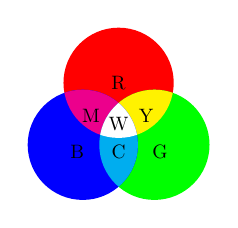
\begin{tikzpicture}[scale=0.35]
		\draw [draw=none, fill=red] (90:1.5) circle (2cm);
		\draw [draw=none, fill=green] (-30:1.5) circle (2cm);
		\draw [draw=none, fill=blue] (210:1.5) circle (2cm);
		\begin{scope} % red + green = yellow
		\clip (90:1.5) circle(2cm);
			\draw [draw=none, fill=yellow] (-30:1.5) circle (2cm);
		\end{scope} % blue + red = magenta
		\begin{scope}
			\clip (210:1.5) circle(2cm);
			\draw [draw=none, fill=magenta] (90:1.5) circle (2cm);
		\end{scope}
		\begin{scope} % green + blue = cyan
			\clip (-30:1.5) circle(2cm);
			\draw [draw=none, fill=cyan] (210:1.5) circle (2cm);
		\end{scope}
		
		% Draw the center area which consists of all the primary colors.
		\begin{scope} % red + green + blue = white
			\clip (90:1.5) circle(2cm);
			\clip (210:1.5) circle(2cm);
			\draw [draw=none, fill=white] (-30:1.5) circle (2cm);	
		\end{scope}
		\node [scale=0.7] at (0,0) {W};
		\node [scale=0.7] at (1,0.3) {Y};
		\node [scale=0.7] at (-1,0.3) {M};
		\node [scale=0.7] at (0,-1) {C};
		\node [scale=0.7] at (-1.5,-1) {B};
		\node [scale=0.7] at (1.5,-1) {G};
		\node [scale=0.7] at (0,1.5) {R};
	\end{tikzpicture}\hfill
	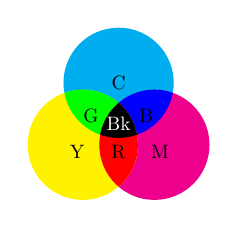
\begin{tikzpicture}[scale=0.35]
		\draw [draw=none, fill=cyan] (90:1.5) circle (2cm);
		\draw [draw=none, fill=magenta] (-30:1.5) circle (2cm);
		\draw [draw=none, fill=yellow] (210:1.5) circle (2cm);
		\begin{scope} % cyan + magenta = blue
		\clip (90:1.5) circle(2cm);
			\draw [draw=none, fill=blue] (-30:1.5) circle (2cm);
		\end{scope} % yellow + cyan = green
		\begin{scope}
			\clip (210:1.5) circle(2cm);
			\draw [draw=none, fill=green] (90:1.5) circle (2cm);
		\end{scope}
		\begin{scope} % magenta + yellow = red
			\clip (-30:1.5) circle(2cm);
			\draw [draw=none, fill=red] (210:1.5) circle (2cm);
		\end{scope}
		
		% Draw the center area which consists of all the primary colors.
		\begin{scope} % cyan + magenta + yellow = black
			\clip (90:1.5) circle(2cm);
			\clip (210:1.5) circle(2cm);
			\draw [draw=none, fill=black] (-30:1.5) circle (2cm);	
		\end{scope}
		\node [scale=0.7, color=white] at (0,0) {Bk};
		\node [scale=0.7] at (1,0.3) {B};
		\node [scale=0.7] at (-1,0.3) {G};
		\node [scale=0.7] at (0,-1) {R};
		\node [scale=0.7] at (-1.5,-1) {Y};
		\node [scale=0.7] at (1.5,-1) {M};
		\node [scale=0.7] at (0,1.5) {C};
	\end{tikzpicture}\hfill
	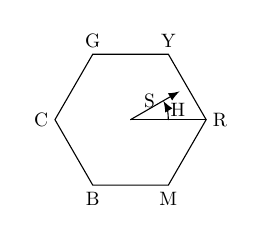
\begin{tikzpicture}[scale=1.2, cap=round,>=latex]
		% Radius of regular polygons
		  \newdimen\R
		  \R=0.8cm
		  \coordinate (center) at (0,0);
		 \draw (0:\R)
		     \foreach \x in {60,120,...,360} {  -- (\x:\R) }
		              -- cycle (300:\R) node[below, scale=0.7] {M}
		              -- cycle (240:\R) node[below, scale=0.7] {B}
		              -- cycle (180:\R) node[left, scale=0.7] {C}
		              -- cycle (120:\R) node[above, scale=0.7] {G}
		              -- cycle (60:\R) node[above, scale=0.7] {Y}
		              -- cycle (0:\R) node[right, scale=0.7] {R};
		   %\draw { (center) -- (0:\R) (center) -- (120:\R) (center) -- (240:\R)};
		   %\draw [densely dashed] { (center) -- (60:\R)  (center) -- (180:\R)  (center) -- (300:\R) };
		   \draw { (center) -- (0:\R) (center) };
		   \draw [->] { (center) -- (30:6mm)};
		   \draw [->] (4mm,0) arc (0:30:4mm);
		   \node [scale=0.7] at (5mm,1mm) {H};
		   \node [scale=0.7] at (2mm,2mm) {S};
		   %\node [fill=white, scale=0.7] at (0,0) {W};
	\end{tikzpicture}\hfill \null
	
	
	\textbf{Color Complements}\\
	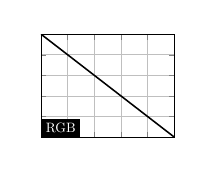
\begin{tikzpicture}[scale=0.7]
		\begin{axis}[tiny, grid=both, xmin=0,ymin=0,
		xmax=1,ymax=1, xticklabel={\empty}, yticklabel={\empty}]
			\addplot[domain=0:1,thick] (x,1-x);
			\node[anchor=south west, color=white, fill=black, scale=0.7] at (axis cs:0,0) {RGB};
		\end{axis}
	\end{tikzpicture}
	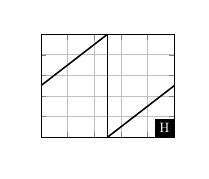
\begin{tikzpicture}[scale=0.7]
		\begin{axis}[tiny, grid=both, xmin=0,ymin=0,
		xmax=1,ymax=1, xticklabel={\empty}, yticklabel={\empty}]
			\addplot[domain=0:0.5,thick] (x,0.5+x);
			\addplot[domain=0.5:1,thick] (x,-0.5+x);
			\addplot[domain=0:1,thick] (0.5,x);
			\node[anchor=south east, color=white, fill=black, scale=0.7] at (axis cs:1,0) {H};
		\end{axis}
	\end{tikzpicture}
	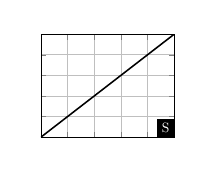
\begin{tikzpicture}[scale=0.7]
		\begin{axis}[tiny, grid=both, xmin=0,ymin=0,
		xmax=1,ymax=1, xticklabel={\empty}, yticklabel={\empty}]
			\addplot[domain=0:1,thick] (x,x);
			\node[anchor=south east, color=white, fill=black, scale=0.7] at (axis cs:1,0) {S};
		\end{axis}
	\end{tikzpicture}	
	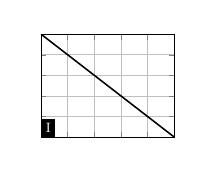
\begin{tikzpicture}[scale=0.7]
		\begin{axis}[tiny, grid=both, xmin=0,ymin=0,
		xmax=1,ymax=1, xticklabel={\empty}, yticklabel={\empty}]
			\addplot[domain=0:1,thick] (x,1-x);
			\node[anchor=south west, color=white, fill=black, scale=0.7] at (axis cs:0,0) {I};
		\end{axis}
	\end{tikzpicture}
	

	
	\section{Image compression}
	\begin{tabularx}{\columnwidth}{l X}
		Relative data redundancy:& $R_D = 1 - { 1 \over C_R }$\\
		Compression ratio: & $C_R = { n_1 \over n_2 }$
	\end{tabularx}
	
	\begin{enumerate}
		\item lossless: text, file
		\item lossy: multimedia data
	\end{enumerate}
	\textbf{Data Redundancies:}
	\begin{enumerate}
		\item Coding (i.e., variable length coding: Entropy coding)
		\item Interpixel (i.e., mapping: Run-Length coding, Predictive coding, DCT, PCA, KLT, Welsh)
		\item Psychovisual (i.e., quantization:): image data that is ignored by the human visual system
	\end{enumerate}
	Objective fidelity criterion between the original image $ f(x,y) $ and the reconstructed output image $ \hat{f}(x,y) $\\
	Root-mean ($ M \times N $ image):\\
	$e_{rms} = \left[ {1 \over MN} \sum_{x=0}^{M-1} \sum_{y=0}^{N-1} [\hat{f}(x,y) - f(x,y) ]^2 \right]^{1/2}$
	
	mean-square SNR:\\
	$SNR_{ms} = { {\displaystyle \sum_{x=0}^{M-1} \sum_{y=0}^{N-1}} \hat{f} (x,y)^2 \over {\displaystyle \sum_{x=0}^{M-1} \sum_{y=0}^{N-1}} [\hat{f}(x,y)- f(x,y)]^2 }$

	Entropy of a random source:
	$H = - \sum_{j=1}^J P(a_j) \log P(a_j)$

	Unitary Transform???????????
	
	\section{Morphological Image Processing}
	\setlength{\gapspace}{0.4\columnwidth}
	\tab{Translation} $(B)_z=\{ w | w=b+z, \mathsf{for} b \in B\}$\\
	\tab{Reflection} $\hat{B}=\{ w | w=-b, \mathsf{for} b \in B\}$\\
	\tab{Complement} $A^c=\{ w | w \notin A\}$\\
	\tab{Difference} $A-B=\{ w | w \in A, w \notin B\}=A \cap B^c$\\
	\tab{Dilation} $A \oplus B=\{z|(\hat{B}_z) \cap A \neq \varnothing \}$\\
	\tab{Erosion} $A \ominus B=\{z|(B)_z \subseteq A\}$\\
	\tab{Opening} $A \circ B = (A \ominus B) \oplus B$\\
	\tab{Closing} $A \bullet B = (A \oplus B) \ominus B$\\
	\tab{Hit-or-Miss} $A \circledast B = (A \ominus B_1) \cap (A^c \ominus B_2)$\\
	\tab{ } $(A \ominus B_1) - (A \oplus \hat{B}_2)$\\
	\tab{Boundary Extraction} $\beta(A) = A - (A \ominus B)$\\
	\tab{Hole Filling} $X_k = (X_{k-1} \oplus B) \cap A^c$\\
	\tab{Connected Components} $X_k = (X_{k-1} \oplus B) \cap A$\\
		%Convex Hull \formelbuch{647}, Thinning \formelbuch{649}, Thickening \formelbuch{650},
        %Skeletons \formelbuch{651}, Pruning \formelbuch{654}
	\tab{Geodesic Dilation} $D_G^{(1)}(F) = (F \oplus B) \cap G$ \\
	\tab{} $D_G^{(n)}(F) = D_G^{(1)}[D_G^{(n-1)}(F)]$\\
	\tab{} $D_G^{(0)}(F)=F$\\
	\tab{Geodesic Erosion} $E_G^{(1)}(F) = (F \ominus B) \cup G$\\
	\tab{} $E_G^{(n)}(F) = E_G^{(1)}[E_G^{(n-1)}(F)]$\\
	\tab{} $E_G^{(0)}(F)=F$\\
	\tab{Recon by Dilation} $R_G^D(F) = D_G^{(k)}(F)$\\
	\tab{Recon by Erosion} $R_G^E(F) = E_G^{(k)}(F)$\\

	\textbf{Dualities:}
	\begin{itemize}
		\item Erosion \& Dilation: $(A \ominus B)^c = A^c \oplus \hat{B}$ ,$(A \oplus B)^c = A^c \ominus \hat{B}$
		\item Opening \& Closing: $(A \bullet B)^c = (A^c \circ \hat{B})$, $(A \circ B)^c = (A^c \bullet \hat{B})$
	\end{itemize}
	
	
	
	gray:
	$b^=b(-x,-y)$
	$f^c=-f(x,y)$
	
	
	\section{Image Segmentation}
	monochrom image segmentation
		
	edge-based
	
	region-based
	\begin{enumerate}
		\item First-order derivatives generally produce thicker edges in an image.
		\item Second-order derivatives have a stronger response to fine details, such as thin lines and isolated points.
		\item First order derivatives generally have a stronger response to a gray-level step.
		\item Second-order derivative	produce a double response at step changes in gray level.
		\item Second-order derivative is more sensitive to noise.
	\end{enumerate}
	edge models:
	\begin{itemize}
		\item Step
		\item Ramp
		\item Roof
	\end{itemize}
	
	fig 10.12\\
	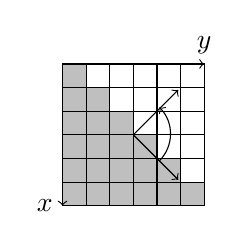
\begin{tikzpicture}[scale=0.3]
		\foreach \x in {0,...,5}
		\foreach \y in {0,...,\x}
			\fill[gray!50](6-\x-1,\y) rectangle (6-\x,\y+1);
		
		\draw [step=,draw=black] (0,0) grid  (6,6) rectangle (0,0);
		
		\draw [->] { (3,3) -- (4.9,1.1)};
		\draw [->] { (3,3) -- (4.9,4.9)};
		\draw [->] (3+1.1,3-1.1) arc (-45:45:1.6);
		   
		\draw[->] (0, 6) -- (6,6) node[above] {$y$};
		\draw[<-] node[left] {$x$}  (0, 0) -- (0,6) ;
	\end{tikzpicture}
	
	\subsubsection*{Line Detection}

		\centerline{
		\begin{mask}
		\hline
		-1 & -1 & -1 \\ \hline
		 2 &  2 &  2 \\ \hline
		-1 & -1 & -1 \\ \hline
		\multicolumn{3}{c}{\scriptsize Horizontal}
		\end{mask}
		\hspace{0.1in}
		\begin{mask}
		\hline
		-1 & -1 &  2 \\ \hline
		-1 &  2 & -1 \\ \hline
		 2 & -1 & -1 \\ \hline
		\multicolumn{3}{c}{\scriptsize $ +45^{\circ} $}
		\end{mask}
		\hspace{0.1in}
		\begin{mask}
		\hline
		-1 &  2 & -1 \\ \hline
		-1 &  2 & -1 \\ \hline
		-1 &  2 & -1 \\ \hline
		\multicolumn{3}{c}{\scriptsize Vertical}
		\end{mask}
		\hspace{0.1in}
		\begin{mask}
		\hline
		 2 & -1 & -1 \\ \hline
		-1 &  2 & -1 \\ \hline
		-1 & -1 &  2 \\ \hline
		\multicolumn{3}{c}{\scriptsize $ -45^{\circ} $}
		\end{mask}}
		$ |R_i | > |R_j| $ for all $ j \neq i $: point associated with line in
		direction of mask $ i $
	
	\centerline{
	\renewcommand{\tabcolsep}{3pt} 
	\begin{mask}
	\hline
	0 & 1 & 0 \\ \hline
	1 & -4 & 1 \\ \hline
	0 & 1 & 0 \\ \hline
	\multicolumn{3}{c}{\scriptsize Laplacian}
	\end{mask}
	\begin{mask}
	\hline
	1 & 1 & 1 \\ \hline
	1 & -8 & 1 \\ \hline
	1 & 1 & 1 \\ \hline
	\multicolumn{3}{p{30pt}}{\scriptsize {Diagonal \newline Laplacian} }
	\end{mask}
	\begin{mask}
	\hline
	-1 & -2 & -1 \\ \hline
	0 & 0 & 0 \\ \hline
	1 & 2 & 1 \\ \hline
	\multicolumn{3}{c}{\scriptsize Sobel}
	\end{mask}
	\begin{mask}
	\hline
	-1 & -1 & -1 \\ \hline
	0 & 0 & 0 \\ \hline
	1 & 1 & 1 \\ \hline
	\multicolumn{3}{c}{\scriptsize Prewitt}
	\end{mask}
	}
		
	LoG: $\Delta^2 G(x,y) = - \left[ \frac{x^2 + y^2 - 2\sigma^2}{\sigma^4 } \right]
	e ^{-\frac{x^2 + y^2}{2 \sigma^2 }}$

	\subsubsection*{Marr-Hildreth}
	\begin{enumerate}
		\item Smooth image with an $nxn$ Gaussian lowpass filter. {\tiny $n$ is the smallest odd integer greater than or equal to $6\sigma$}.
		\item Compute the Laplacian of smoothed image.
		\item Find the zero crossing.
	\end{enumerate}
		
	\subsubsection*{Canny Edge Detector}
	\begin{enumerate}
		\item Image smoothed by Gaussian filter
		\item Local gradient computed
		\item Apply nonmaxima suppression to gradient magnitude image
		\item Use double thresholding and connectivity analysis to \textit{detect} and \textit{link} edges.
	\end{enumerate}
	
	\section{Representation and Description}
	
	Representation
	Boundary Descriptors
	Regional Descriptors: 
	 simple:area, perimeter, compactness, circularity ratio
	 topological: 
	 texture: GLCM
	
% You can even have references
\vspace{5mm}
\rule{0.3\linewidth}{0.25pt}
\scriptsize

\textbf{References:}
\begin{itemize}[leftmargin=2em]
	\item [{[1]}] Digital Image Processing, by Gonzalez and Woods
\end{itemize}
Made by \href{http://webpages.iust.ac.ir/mehralian/}{ma.mehralian} using \LaTeX
\end{multicols}

\end{document}